% !Mode:: "TeX:UTF-8"
\documentclass[type=doctor, openany, pifootnote, nocolor]{shuthesis}
\usepackage{pdfpages}
\usepackage{shuthesis}
\usepackage{times}

\usepackage{bm}

\usepackage{algorithm}
\usepackage{algorithmic}

\floatname{algorithm}{算法}  
\renewcommand{\algorithmicrequire}{\textbf{输入:}}  
\renewcommand{\algorithmicensure}{\textbf{输出:}} 

\graphicspath{{figures/}}

\usepackage{listings}
\renewcommand{\lstlistingname}{代码}
\newfontfamily\courier{Courier New}
\lstset{linewidth=1.1\textwidth,
        numbers=left, %设置行号位置 
        basicstyle=\small\courier,
        numberstyle=\tiny\courier, %设置行号大小  
        keywordstyle=\color{blue}\courier, %设置关键字颜色  
        %identifierstyle=\bf,
        commentstyle=\it\color[cmyk]{1,0,1,0}\courier, %设置注释颜色 
        stringstyle=\it\color[RGB]{128,0,0}\courier,
        %framexleftmargin=10mm,
        frame=single, %设置边框格式  
        backgroundcolor=\color[RGB]{245,245,244},
        %escapeinside=``, %逃逸字符(1左面的键),用于显示中文  
        breaklines, %自动折行  
        extendedchars=false, %解决代码跨页时,章节标题,页眉等汉字不显示的问题  
        xleftmargin=2em,xrightmargin=2em, aboveskip=1em, %设置边距  
        tabsize=4, %设置tab空格数  
        showspaces=false %不显示空格  
        basicstyle=\small\courier
}  

\newenvironment{Solution}
{\color[RGB]{0,69,128}{\textbf{解}:} \kaishu\color[RGB]{0,69,128} }


\begin{document}


~

\vspace{10mm}


\begin{figure}[!htbp]
    \centering
    
\includegraphics[width=10cm]{shulogo.png}
\end{figure}


\centerline{\xiaoer{\textbf{SHANGHAI  UNIVERSITY}}}

\vspace{8mm}

\centerline{\kaishu{\xiaoyi{\textbf{<信息安全技术>实验报告}}}}

\vspace{8mm}

% \renewcommand{\thefootnote}{\fnsymbol{footnote}}

\vspace{6cm}

\begin{table}[!htbp]\large
    \centering
    \begin{tabular}{r c}
        学~~~~~~~~院    & 计算机工程与科学学院\\  \cmidrule(l){2-2} 
        学~~~~~~~~号    & yb yb\\               \cmidrule(l){2-2} 
        姓~~~~~~~~名    & yb yb\\            \cmidrule(l){2-2} 
    \end{tabular}
\end{table}

\frontmatter
{
    \hypersetup{linkcolor=black}
    \tableofcontents
}

\mainmatter
\chapter{Shamir 秘密共享}

\section{实验目的}

巩固对Shamir秘密共享算法的理解。

\section{实验要求}

实现一个(k,n)-Shamir 秘密共享方案,其中k=3,n=5,包含以下功能:
\begin{enumerate}
    \item 给定一个数字,可以计算出对应的share
    \item 给定k个share, 能够重构出秘密值。
\end{enumerate}

\section{实验内容}

\subsection{Shamir 秘密共享算法分析}

Shamir的秘密共享方案是由Adi Shamir提出的最早的秘密共享算法,
它的实现基于有限域上多项式的插值\cite{contributors_2019}。

此处我们不加证明的给出Langrange插值定理。

\begin{theorem}
    \label{the:lang}
    给定$n$个互异点$P_i=(x_i,y_i)\in \mathbb{F}^2,\forall x_i \neq x_j, i \neq j,0\leq i,j < n$,
    则可唯一确定$n-1$阶多项式$f(x)\in \mathbb{F}[x]$,且有:
    \begin{equation*}
        f(x) = \sum_{i=1}^{n} y_i \left(
            \prod_{j\neq i}^{1\leq j \leq n}\frac{x-x_j}{x_i-x_j}
        \right)
    \end{equation*}
\end{theorem}

根据秘密共享的要求,给定$(k,n)$秘密共享方案,则需要被共享的数据
被分为$n$份share,其中任意$k$或多于$k$份share都能还原本来的数据,
而任意少于$k$份share都不包含原来数据的任何信息。

因此,我们可以这样设计基于多项式插值的秘密共享方案:
\begin{enumerate}
    \item \textbf{多项式准备}:以常数项为数据,随机生成有限域$\mathbb{F}$上的多项式$f(x)$;
    \item \textbf{数据分割}:生成多项式$f(x)$上的$n$个互异点,将其坐标信息打包为share;
    \item \textbf{数据重构}:利用$k$个share中的坐标信息进行多项式插值,重构原来的多项式$f(x)$,取其常数项$f(0)$即为还原的数据。
\end{enumerate}

\newpage
\subsection{程序设计与实现}

    具体代码见附录\ref{appendix:Shamir},此处仅对关键设计进行说明。

\subsubsection{Element类设计}

根据上文可以知道,所给的插值方法是在有限域上进行的,因此笔者设计了Element类
来封装有限域$\mathrm{GF}(2^{128})$上的元素运算。

其中设置有限域为$\mathrm{GF}(2^{128})$的原因是,它可以表示128bit的信息,
而目前的AES加密算法的密钥长度最小即为128bit,因此该方案在实现后可以用于
对AES密钥的共享。而在需要共享数据时,就可先用AES对其进行加密,并把密文放置在
公共空间中,通过分发AES密钥的share来缩短share长度,并实现相同效果。

此外,该类重构了乘法,加法和幂次运算,并且基于扩展欧几里得算法设计了求模逆元的方法。
具体在求模数时,查表得到$\mathrm{GF}(2^{128})$的一个本原多项式
$1+x+x^2+x^7+x^{128}$,
即可取模数irr\_poly为$1 + 2 + 4 + 128 + 2 ^ {128}$。

\subsubsection{Shamir类设计}

Shamir类包含了split和combine两个静态方法。

\textbf{数据分割}:split方法即为数据分割,要求传入方案参数$k, n$以及要分割的数据secret。
在多项式准备过程中,通过Crypto库的Random类生成伪随机数(保证其为PRG生成),
将常数项设置为分割数据secret。

取点过程中直接取$x_i = 1, 2, \cdots, n, 0\leq i < n$,通过迭代运算得到$y_i$。
最后打包为Python中的列表对象返回shares。

\textbf{数据重构}:combine方法即为数据重构,要求传入shares。不要求给定
原来的方案参数,因为当shares的数目$m<k$时,插值得到多项式错乱,无需要信息,
而$m>k$时,由于点$P_k, P_{k+1}, \cdots, P_m$仍在前$k$个点还原的多项式上,
因此最后的插值结果不会发生改变。

具体在计算中即利用了定理\ref{the:lang}中的公式,不再说明。

\newpage
\subsubsection{图形化界面设计}

如下图\ref{fig:shamir}所示即为设计的3,5-Shamir秘密共享方案图形化界面,
设计用到Python的PyQt5库。

\begin{figure}[!htbp]
    \centering
    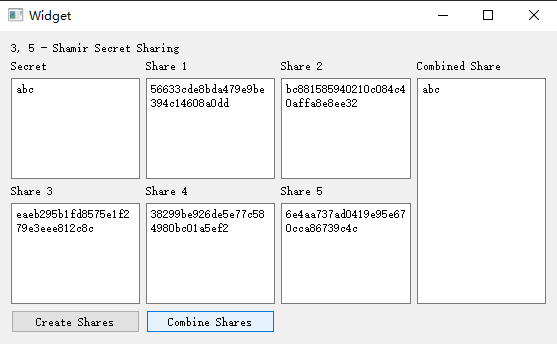
\includegraphics[width=0.7\textwidth]{figures/shamir.png}
    \caption{3,5-Shamir秘密共享方案的图形化界面}
    \label{fig:shamir}
\end{figure}

给定文本框Secret中的内容,点击Create Shares即可获得5份share
(share通过binascii库的hexlify函数转化为16进制格式),或者输入
5份share后,点击Combine Shares即可在文本框Combined Share显示原来的数据内容。

其中,combine过程的share选择取决于文本框Share 1-5是否有内容,如有则会提取。
由于选定门限为3,5,因此3份或以上的share可以还原,少于3份则会显示为NULL,如下图\ref{fig:shamir_2}所示。

\begin{figure}[!htbp]
    \centering
    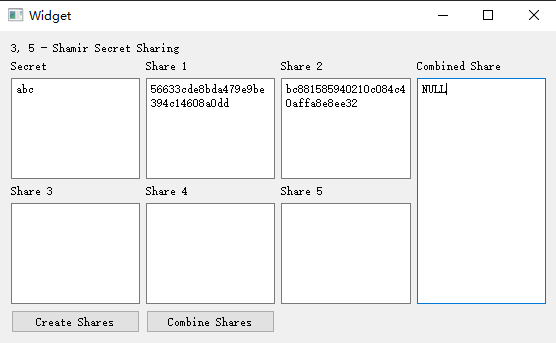
\includegraphics[width=0.7\textwidth]{figures/shamir_2.png}
    \caption{3,5-Shamir秘密共享方案恢复失败的结果}
    \label{fig:shamir_2}
\end{figure}

\subsection{图像秘密共享方案的讨论}

该处给出了一种基于上文所给的Shamir秘密共享的图像秘密共享方案。
我们知道图像在计算机存储时可认为是二维矩阵的存储,因此只需要将
矩阵中的每一个元素进行秘密共享,即可对原本的图像进行共享。
最终结果如图\ref{fig:shamir_3}所示。

\begin{figure}[!htbp]
    \centering
    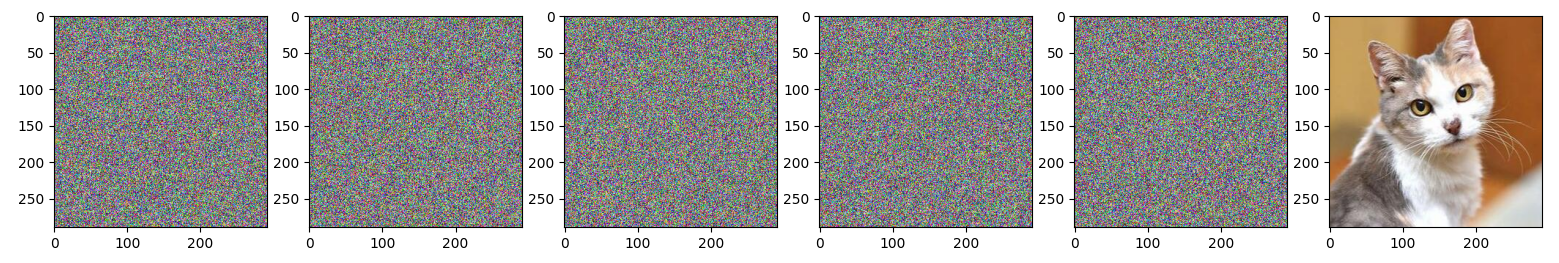
\includegraphics[width=1\textwidth]{figures/shamir_3.png}
    \caption{3,5-图像秘密共享方案的结果}
    \label{fig:shamir_3}
\end{figure}

可看到图\ref{fig:shamir_3}中前五张图即为原本的秘密共享结果,图像和噪点图类似。
任取前5张图中的3张以上图片即可还原出第六张图片。

对于一张$n\times n$像素的彩图,需要进行$4n^2$次秘密共享,因此该方法的效率
还是较低的。从改进角度考虑,可将原本的有限域取为$\mathrm{GF}(2^8)$即可
完成RGB图像编码的数值范围要求,从而降低生成多项式的阶数来提高效率。

此外由于产生的图像类似于噪点图,可作为滤镜作用于其他图像上,最后通过提取算法
即可进行share的隐秘化。
\chapter{Many Time Pad}

\section{实验目的}

我们已经证明一次一密在已知密文攻击下是安全的。本次实验将尝试探索当密钥被重复使用时的已知密文攻击方法。

\section{实验要求}
如下所示是11个使用同一个密钥按照one time pad方法进行加密得到的密文。
请使用前10个密文进行分析,并对目标密文进行解密。
其中消息是[a-zA-Z]以及空格组成的字符,使用ascii编码,密文使用hex编码。

\section{实验内容}

\subsection{攻击思路}

此处的攻击思路参考了Ruan的文章\cite{ruan_2020}。

MTP的不安全性来源于ASCII编码的性质。给定密文$c_1,c_2$、明文$m_1,m_2$和密钥$k$,
根据加密方案和异或运算的性质有:
\begin{equation}
    c_1 \oplus c_2 = (m_1 \oplus k) \oplus (m_2 \oplus k) = m_1 \oplus m_2
\end{equation}

而在ASCII编码方案中,空格的字节码为0x20,0x41-0x5A 是大写字母 A-Z,0x61-0x7A 是小写字母 a-z。
发现小写字母异或空格时,恰得到其对应的大写字母,反之亦然。

因此分析密文中的内容,如果某一位为字母,则说明其对应的明文位和密钥位必有一个是其对应大写或小写化的字母,
而另外个是空格。

而对于对条密文的某一位如果大部分为字母,则可以猜测这一位的密钥是空格。

此处,“大部分”被具体定义为猜测阈值,笔者给定猜测阈值为:
\begin{equation}
    threshold = |C| - \sqrt{|C|}
\end{equation}

其中$C$为所给密文集合,该公式没有理论上的依据性,只是恰好得到的结果比较好,实际上还可对其上下调节。

\subsection{程序设计与实现}

具体代码见附录\ref{appendix:mtp},此处仅对关键设计进行说明。

由于所给密文使用了hex编码,因此此处利用了Python binascii库中的
unhexlify函数进行解码,转化为字节串。

\subsection{攻击结果}

最终得到的字符串为:The secuet-message\textbackslash xeeis: Wh\textbackslash x1an usi|g a stream cipher, never\textbackslash xf8use the key more than once
可发现该种攻击方式不能完全还原原来的明文。

但由于自然语言本身具有纠错性,因此可根据上下文语义人工猜测原明文为:The secret message is: When using a stream cipher, never reuse the key more than once.
\chapter{AES}

\section{实验目的}

理解 AES 算法的不同工作模式。

\section{实验要求}
实现两个基于 AES 的加密/解密系统,一个在 CBC 模式下使用 AES,另
一个在 CTR 模式下使用 AES。 在这两种情况下,16 字节的初始向量 IV 都
是随机选择的,并已放在密文中。对于 CBC 加密,请使用课程中讨论的 PKCS5
填充方案。
以下提供了解密过程正确性的测试用例。测试用例包含了 AES 密钥和一个
密文(两者都是十六进制编码的),需要恢复出明文并在实验报告中展示结果。

\section{实验内容}


\subsection{程序设计与实现}

具体代码见附录\ref{appendix:aes},此处仅对关键设计进行说明。

由于需要对分组进行异或或者数加操作,笔者定义了函数byte\_xor和byte\_add。

由于需要使用PKCS5填充方案,笔者定义了函数msg\_block\_generator和cipher\_block\_generator
用于填充。

笔者给出两个类CBC和CRT分别代表两种分组模式,包含方法encrypt和decrypt。
如图\ref{fig:aes}所示,以ECB, CRT和CBC的加密模式为例,可以看到ECB模式中的分组加密可以应用到
CTR模式和CBC模式中。按照实验要求,在CRT模式和CBC模式的加密过程中,
可直接调用Crypto库中的AES类使用其ECB模式块进行代码简化。解密同理。

\begin{figure}[!htbp]
    \centering
    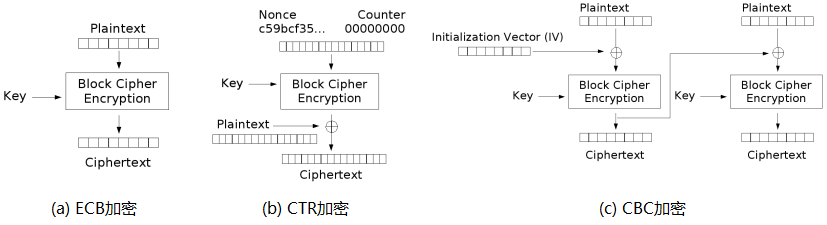
\includegraphics[width=1\textwidth]{figures/aes.png}
    \caption{ECB, CRT, CBC加密模式对比}
    \label{fig:aes}
\end{figure}

\subsection{恢复明文结果}

四组数据的解密结果分别为:

Basic CBC mode encryption needs padding.

Our implementation uses rand. IV

CTR mode lets you build a stream cipher from a block cipher.

Always avoid the two time pad!
\setcounter{chapter}{3}
\chapter{视频流Hash}

\section{实验目的}
练习抗碰撞哈希函数的使用,理解哈希函数抗碰撞的安全性。

\section{实验要求}

(前略)...网站不计算整个文件的哈希值,而是将文件分成 1KB 的数据块
(1024 字节)。它计算最后一个块的哈希并将值
附加到倒数第二个块。然后它计算这个增强的倒数第二个块的散列,并将得到
的散列附加到最后的第三个块。此过程从最后一个块继续到第一个块,如下图
所示:

\begin{figure}[!htbp]
\centering
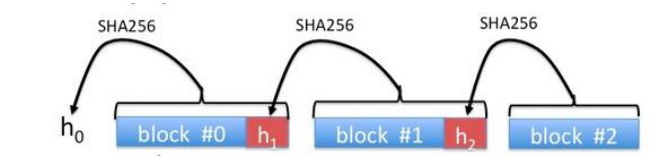
\includegraphics[width=0.8\textwidth]{hash.png}
\end{figure}

网站将最终的哈希值$h_0$通过认证信道分发给用户。

在用户端,浏览器每次下载文件$F$的一个数据块,以及上述所示的附加哈希
值,并进行验证,若验证通过则播放第一个视频块。具体的,通过验证
$H(B_0||h_1)$与$h_0$是否相等来验证第一个区块的完整性; 
通过验证$H(B_1||h_2)$与$h_1$
是否相等来验证第二个区块的完整性;以此类推直至最后一个区块。这样,每
个块都会在收到时进行验证和播放,无需等到整个文件下载完毕。容易证明,
只要哈希函数满足抗碰撞性质,那么攻击者的篡改行为无法通过上述完整性验
证。

本次实验使用 SHA-256 作为哈希函数,实现上述视频验证程序。每一个
哈希值以二进制数据的形式和视频数据块进行链接。若视频数据大小不是 1KB
的整倍数,那么最后一个区块可以小于 1KB,其余的数据区块则需要刚好是
1KB 的整倍数。

程序能够根据输入的文件 $F$计算得到相应的$h_0$,以验证收到文件的正确
性。具体的,请在实验报告中给出视频 1 的$h_0$值(使用 hex 编码)。

\newpage
\section{实验内容}

本实验通过Python语言编写脚本进行,下面具体说明。

\subsection{文件读取}

实验中给到的文件为视频格式,可通过Python语言os库分块读取。

笔者设计了get\_file\_block函数用于进行读取,代码如下:

\begin{lstlisting}[language = Python]
def get_file_block(file_name):
    with open(file_name, 'rb') as f:
        for idx in reversed(range(0, os.path.getsize(file_name), BLOCK_SIZE)):
            f.seek(idx)
            yield f.read(BLOCK_SIZE)
\end{lstlisting}

其中BLOCK\_SIZE为全局变量,定义为1024,通过该函数即可以1 KB的大小,分块读取视频文件。

值得一提的是,笔者使用yield语法进行结果返回,使得函数成为生成器(Generator),可模拟
视频流在实际环境中分块送达的特点。

\subsection{分块哈希}

该部分使用了Crypto库中的SHA256算法,具体代码如下:

\begin{lstlisting}[language = Python]
def stream_hash(file_name):
    hash_result = b''
    for block in get_file_block(file_name):
        h = SHA256.new(block + hash_result) ## Note:1
        hash_result = h.digest()
    return h.hexdigest()
\end{lstlisting}

可注意在Note:1所在行,我们对每块内容加上上一块的哈希值,作为哈希函数的输入,进行计算。

最后返回的哈希值为视频文件的哈希值的hex编码形式。

\section{实验结果}

对于验证性视频6.2.birthday.mp4,得到的哈希值与所给测试结果相同,为:
\begin{center}
    03c08f4ee0b576fe319338139c045c89c3e8e9409633bea29442e21425006ea8
\end{center}

并计算视频6.1.intro.mp4,得到的哈希值为:
\begin{center}
    5b96aece304a1422224f9a41b228416028f9ba26b0d1058f400200f06a589949
\end{center}
\chapter{Padding Oracle攻击}

\section{实验目的}

理解 padding oracle 攻击的过程,验证攻击的可行性。

\section{实验准备}

网站 crypto-class.appspot.com 部署了一个填充预言机的模拟示例,请搭建
可以访问上述地址的实验环境。

\section{实验要求}

假设攻击者想要利用上述网站的返回结果窃取信息。攻击者通过观察得
知:网站将用户的数据加密后利用 URL 参数进行传输,例如:

\begin{center}
    http://crypto-class.appspot.com/po?er=f20bdba6ff29eed7b046d1df9fb7000
\end{center}

当用户 Alice 和网站进行交互时,网站将上述 URL 发送给 Alice。攻击者
猜测在"po?er="这一 URL 变量的值可能 Alice 会话中的一个一些秘密数据。该
数据使用 AES CBC(随机初始向量加密)模式进行加密并将加密结果使用
hex 进行编码。攻击者发现上述网站存在 padding oracle 攻击:当解密的
CBC 密文出现填充错误时,网站服务器返回 403 错误(forbidden request),
当 CBC 填充合法,但是 MAC 验证失败时,网站返回 404 错误(URL not 
found)。

请利用以上信息,解密上述代码框中的密文。为了完成解密,你可以发送
任意的如下格式的 HTTP 请求并获取其对用的错误代码。Padding oracle 可以
进行逐字节的解密,你需要发送 256 个 HTTP 请求来完成一个字节的解密。需
要注意的时密文的第一个分组是随机的初始向量,且解密得到的消息使用
ASCII 编码。

\begin{center}
    http://crypto-class.appspot.com/po?er=
\end{center}

\newpage
\section{实验内容}

\subsection{攻击方法分析}

如下图,为CBC模式下的解密示意图。

\begin{figure}[!htbp]
    \centering
    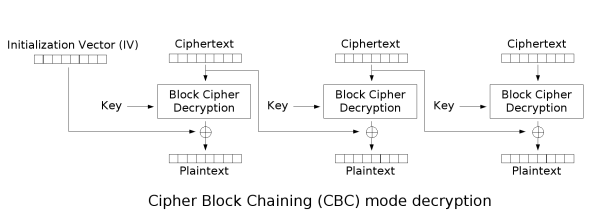
\includegraphics[width=0.9\textwidth]{cbc.png}
    \caption{CBC模式下的解密示意图}
\end{figure}
 
形式化的可以写为$P_i = D(K,C_i) \oplus C_{i-1}$,且有$C_0 = IV$。

在AES中,分块长度为16字节,当最后一块不够,或正好是16字节时,需要填充,规则为PKCS5。

此时,我们截获了密文$Y$,并想获得密文$Y$的最后一个字节。我们构造密文$F|Y$,那么服务器
在进行解密时,有$P=D(K,Y)\oplus F$,此时我们通过修改密文$F$的最后一个字节,$F_{15}$
就可以修改$Y$对应明文的最后一个字节。

给出对应的攻击过程:
\begin{enumerate}
    \item $i = 0$,$F$为随机字节
    \item $F_{15} = i \oplus 0x01$
    \item 将$F|Y$发送给服务器,若$P$的最后一个字节是$i$,则最后Padding为$0x01$,无错误,
    否则只有$P$最后$P_{15} \oplus i \oplus 0x01$字节都是$P_{15} \oplus i \oplus 0x01$
    才不会报错,此时满足的概率是小的,我们认为攻击成功。
    \item 若不满足,$i = i+1$,返回到第2步。
\end{enumerate}

当获取了最后一个字节,固定好后继续设置$F_{14}=i\oplus 0x02$就可继续获取倒数第二个字节,以此类推。

此处需要注意在猜测填充块(即最后一块)的倒数第一个字节时,若第3步不报错,需要修改IV的倒数第二个字节
打破填充规则,若此时仍然Padding正常,则说明猜测准确,否则需要继续猜测其他值。

(此处主要参考了CTF-Wiki中的攻击模式说明\footnote{https://ctf-wiki.org/crypto/blockcipher/mode/padding-oracle-attack})

\subsection{攻击结果}
由于实验环境特殊性,笔者根据mithi的工作\footnote{https://github.com/mithi/simple-cryptography/tree/master/04-padding-oracle}
在本地搭建了Padding Oracle攻击环境。

攻击结果:
\begin{lstlisting}
Case A
--------------
SERVER > localhost:9000
TARGET > 4ca00ff4c898d61e1edbf1800618fb2828a226d160dad07883d
04e008a7897ee2e4b7465d5290d0c0e6c6822236e1daafb94ffe0c5da05d
9476be028ad7c1d81
PLAINTEXT > Basic CBC mode encryption needs padding.
\end{lstlisting}
\chapter{RSA攻击}

\section{实验目的}

本次实验的目的是探索 RSA 在不正确生成模 $N$ 的情况下的安全性。

\section{实验要求}

在 RSA 的密钥生成阶段,不同用户应该独立的生成模 $N$,即选取大素数 $p$ 和 $q$
相乘得到 $N$。假设某个项目中的 RSA 具体实现过程如下:1)首先随机选取一
个随机数 $R$ 然后选取距离 $R$ 最近的素数 $p$,以及另外一个相近的素数 $q$。2)$p$
和 $q$ 相乘得到 $N$。由于 $p$ 和 $q$ 为相近的两个素数,在此情况下存在对 $N$ 的高效
分解方法,导致方案不安全。

假设$N$的因子$p$和$q$满足:
\begin{equation}
    \label{eq:pq}
    |p-q|<2N^{1/4}
\end{equation}

那么$N$的分解可由如下分析得出:

令$A=(p+q)/2$,那么根据式\ref{eq:pq},能够得到$A-\sqrt{N}<1$。
因此可以根据$A=\left\lceil \sqrt{N}\right\rceil $计算得到$A$。

下图展示了$p,q,\sqrt{N},(p+q)/2$之间的关系。

\begin{figure}[!htbp]
    \centering
    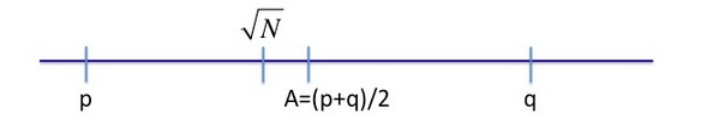
\includegraphics[width=0.8\textwidth]{figures/RSA.png}
\end{figure}

由于$N=pq=(A-x)(A+x)=A^2-x^2$,因此有$x=\sqrt{A^2 - N}$。当求得
$x$以后,容易根据$p=A+x,q=A-x$得到$N$的分解。

根据上述分析,请完成挑战(在实验内容中给出)。

\section{实验内容}

\subsection{分解挑战1}

如下的整数$N$是两个素数$p,q$的乘积,且满足$|p-q|<2N^{1/4}$,请分解
整数N并给出其十进制结果。\\

$
\begin{aligned}
    N = &17976931348623159077293051907890247336179769789423065727343008115 \\
        & 77326758055056206869853794492129829595855013875371640157101398586 \\
        & 47833778606925583497541085196591615128057575940752635007475935288 \\
        & 71082364994994077189561705436114947486504671101510156394068052754 \\
        & 0071584560878577663743040086340742855278549092581
\end{aligned}
$\\

本次实验采用了Python语言编写脚本,并利用了gmpy2库进行大整数的高精度运算。

挑战1的求解代码如下:
\begin{lstlisting}[language = Python]
def factoring_1(N):
    A, r = gmpy2.isqrt_rem(N)   ## 求平方根
    if r > 0:
        A += 1
    A_squared_minus_N = A**2 - N
    x = gmpy2.isqrt(A_squared_minus_N)
    p = A - x
    q = A + x
    N_slash = gmpy2.mul(p, q)
    assert N == N_slash         ## 检查N是否分解成功
    return p, q
\end{lstlisting}

该部分攻击原理实验要求中已经给出,因此不再赘述。

需注意,此处传入的$N$为一个大整数,因此需要使用gmpy2库中的mpz方法初始化。此外,后续的开方,乘法
操作,都需要使用gmpy2库中的各方法进行,否则会引起错误。

最终得到:

$
\begin{aligned}
    p = &134078079299425970995740249982058461274793658205923933777235614437\\
        &217640300736627688911116143623269986750405460943393208384195233759\\
        &86027530441562135724301\\
    q = &134078079299425970995740249982058461274793658205923933777235614437\\
        &217640300737785609803489305577505696600492340021925908230851639400\\
        &25485114449475265364281
\end{aligned}
$\\

\subsection{分解挑战2}

如下的整数$N$是两个素数$p,q$的乘积,且满足$|p-q|<2^{11}N^{1/4}$,请分解
整数N并给出其十进制结果。\\

$
\begin{aligned}
    N = &6484558428080716696628242653467722787263437207069762630604390703787\\
        & 9730861808111646271401527606141756919558732184025452065542490671989 \\
        & 2428844841839353281972988531310511738648965962582821502504990264452 \\
        & 1008852816733037111422964210278402893076574586452336833570778346897 \\
        & 15838646088239640236866252211790085787877
\end{aligned}
$\\

挑战2的求解代码如下:
\begin{lstlisting}[language = Python]
def factoring_2(N):
    N_sqrt, r = gmpy2.isqrt_rem(N)
    if r > 0:
        N_sqrt += 1
    for offset in range(2**20):
        A = N_sqrt + offset
        A_squared_minus_N = A**2 - N
        x = gmpy2.isqrt(A_squared_minus_N)
        p = A - x
        q = A + x
        if gmpy2.mul(p, q) == N:
            break
    return p, q
\end{lstlisting}

此处与挑战1的不同是,$|p-q|$增大了,但仍有$A-\sqrt{N}< 2^20$,可从$\sqrt{N}$开始搜索$A$的值。

我们枚举偏移量$offset \in \left[0, 2^{20}\right)$,尝试利用$p=A+x=A+\sqrt{A^2-N}$对$N$进行分解,
当分解成功时返回$p,q$。

最终得到:

$
\begin{aligned}
    p = &254647961469961834380088165639739422293414542685241578463285819278\\
        &857779699852228351438510732495734541073844615571931733044972448140\\
        &71505790566593206419759\\
    q = &254647961469961834380088165639739422293414542685241578463285819278\\
        &857779701063980544912465269708141676325635095417847347418713798566\\
        &82354747718346471375403
\end{aligned}
$\\

\subsection{解密挑战}

如下所示是使用分解挑战 1 中的模数 N 对一段消息进行加密得到的密文。其中
加密指数 e=65537。明文消息使用 ASCII 进行编码后使用 PKCS v1.5 进行消
息填充,需要指出的是,消息中使用'0x00'对消息和随机填充进行分割,而不
是'0xFF'。请在实验报告中给出下列密文的解密结果。\\

$
\begin{aligned}
    &220964518674103817763065611348834180174100697878928310717318391436761\\
        &356001205380042823296504735094243439462197515122564658399679428894607\\
        &645420405815647489880137348641204523252293201764879166664029975091887\\
        &299716905260832220677716000193292608700095799937240774589677736978175\\
        &71267229951148662959627934791540
\end{aligned}
$\\

由于挑战1中已经对模数$N$进行了分解得到了$p,q$,因此后续进行解密是较为简单的。
具体步骤如下:
\begin{enumerate}
    \item 计算$\varphi(N) = (p-1)(q-1)$;
    \item 计算私钥$d = e^{-1} \bmod \varphi(N)$;
    \item 利用解密公式获得明文消息:$m = c^d \bmod N$。
    \item 找到分割字符'0x00',将明文消息分割为随机填充和消息,获得最后结果。
\end{enumerate}

求解代码如下:
\begin{lstlisting}[language = Python]
def decrypt(c, e, n):
    p, q = factoring_1(n)
    phi_n = gmpy2.mul(p - 1, q - 1)
    d = gmpy2.invert(e, phi_n)
    msg_hex = hex(gmpy2.powmod(c, d, n))[2:]

    ## PKCS v1.5 '0x02'开头,需补位
    if msg_hex[0] == '2':
        msg_hex = '0' + msg_hex
    
    ## 消息分割,取消息,去随机填充
    msg = msg_hex.split('00')[1]

    return str(bytes.fromhex(msg))
\end{lstlisting}

最后得到的消息为:
\begin{center}
    Factoring lets us break RSA.
\end{center}

\bibliographystyle{shuthesis}
\bibliography{reference/refs}

% \backmatter
% \begin{appendix}
% \chapter{实验代码}

\section{Shamir 秘密共享}
\label{appendix:Shamir}

shamir.py

\begin{lstlisting}[language = Python]
from Crypto.Util.py3compat import is_native_int
from Crypto.Util import number
from Crypto.Util.number import long_to_bytes, bytes_to_long
from Crypto.Random import get_random_bytes as rng


def _mult_gf2(f1, f2):
    """Multiply two polynomials in GF(2)"""

    # Ensure f2 is the smallest
    if f2 > f1:
        f1, f2 = f2, f1
    z = 0
    while f2:
        if f2 & 1:
            z ^= f1
        f1 <<= 1
        f2 >>= 1
    return z


def _div_gf2(a, b):
    """
    Compute division of polynomials over GF(2).
    Given a and b, it finds two polynomials q and r such that:

    a = b*q + r with deg(r)<deg(b)
    """

    if (a < b):
        return 0, a

    deg = number.size
    q = 0
    r = a
    d = deg(b)
    while deg(r) >= d:
        s = 1 << (deg(r) - d)
        q ^= s
        r ^= _mult_gf2(b, s)
    return (q, r)


class _Element(object):
    """Element of GF(2^128) field"""

    # The irreducible polynomial defining this field is 1+x+x^2+x^7+x^128
    irr_poly = 1 + 2 + 4 + 128 + 2 ** 128

    def __init__(self, encoded_value):
        """Initialize the element to a certain value.

        The value passed as parameter is internally encoded as
        a 128-bit integer, where each bit represents a polynomial
        coefficient. The LSB is the constant coefficient.
        """

        if is_native_int(encoded_value):
            self._value = encoded_value
        # elif len(encoded_value) == 16:
        else:
            self._value = bytes_to_long(encoded_value)
        # else:
        #     raise ValueError("The encoded value must be an integer or a 16 byte string")

    def __eq__(self, other):
        return self._value == other._value

    def __int__(self):
        """Return the field element, encoded as a 128-bit integer."""
        return self._value

    def encode(self):
        """Return the field element, encoded as a 16 byte string."""
        return long_to_bytes(self._value)

    def __mul__(self, factor):

        f1 = self._value
        f2 = factor._value

        # Make sure that f2 is the smallest, to speed up the loop
        if f2 > f1:
            f1, f2 = f2, f1

        if self.irr_poly in (f1, f2):
            return _Element(0)

        mask1 = 2 ** 128
        v, z = f1, 0
        while f2:
            # if f2 ^ 1: z ^= v
            mask2 = int(bin(f2 & 1)[2:] * 128, base=2)
            z = (mask2 & (z ^ v)) | ((mask1 - mask2 - 1) & z)
            v <<= 1
            # if v & mask1: v ^= self.irr_poly
            mask3 = int(bin((v >> 128) & 1)[2:] * 128, base=2)
            v = (mask3 & (v ^ self.irr_poly)) | ((mask1 - mask3 - 1) & v)
            f2 >>= 1
        return _Element(z)

    def __add__(self, term):
        return _Element(self._value ^ term._value)

    def inverse(self):
        """Return the inverse of this element in GF(2^128)."""

        # We use the Extended GCD algorithm
        # http://en.wikipedia.org/wiki/Polynomial_greatest_common_divisor

        if self._value == 0:
            raise ValueError("Inversion of zero")

        r0, r1 = self._value, self.irr_poly
        s0, s1 = 1, 0
        while r1 > 0:
            q = _div_gf2(r0, r1)[0]
            r0, r1 = r1, r0 ^ _mult_gf2(q, r1)
            s0, s1 = s1, s0 ^ _mult_gf2(q, s1)
        return _Element(s0)

    def __pow__(self, exponent):
        result = _Element(self._value)
        for _ in range(exponent - 1):
            result = result * self
        return result


class Shamir(object):
    """Shamir's secret sharing scheme.

    A secret is split into ``n`` shares, and it is sufficient to collect
    ``k`` of them to reconstruct the secret.
    """

    @staticmethod
    def split(k, n, secret):
        """Split a secret into ``n`` shares.

        The secret can be reconstructed later using just ``k`` shares
        out of the original ``n``.
        Each share must be kept confidential to the person it was
        assigned to.

        Each share is associated to an index (starting from 1).

        Args:
          k (integer):
            The sufficient number of shares to reconstruct the secret (``k < n``).
          n (integer):
            The number of shares that this method will create.
          secret (byte string):
            A byte string of 16 bytes (e.g. the AES 128 key).

        Return (tuples):
            ``n`` tuples. A tuple is meant for each participant and it contains two items:

            1. the unique index (an integer)
            2. the share (a byte string, 16 bytes)
        """

        #
        # We create a polynomial with random coefficients in GF(2^128):
        #
        # p(x) = \sum_{i=0}^{k-1} c_i * x^i
        #
        # c_0 is the encoded secret
        #

        coeffs = [_Element(rng(16)) for i in range(k - 1)]
        coeffs.append(_Element(secret))

        # Each share is y_i = p(x_i) where x_i is the public index
        # associated to each of the n users.

        def make_share(user, coeffs):
            idx = _Element(user)
            share = _Element(0)
            for coeff in coeffs:
                share = idx * share + coeff

            return share.encode()

        return [(i, make_share(i, coeffs)) for i in range(1, n + 1)]

    @staticmethod
    def combine(shares):
        """Recombine a secret, if enough shares are presented.

        Args:
          shares (tuples):
            The *k* tuples, each containin the index (an integer) and
            the share (a byte string, 16 bytes long) that were assigned to
            a participant.
          ssss (bool):
            If ``True``, the shares were produced by the ``ssss`` utility.
            Default: ``False``.

        Return:
            The original secret, as a byte string (16 bytes long).
        """

        k = len(shares)

        gf_shares = []
        for x in shares:
            idx = _Element(x[0])
            value = _Element(x[1])
            if any(y[0] == idx for y in gf_shares):
                raise ValueError("Duplicate share")
            gf_shares.append((idx, value))

        result = _Element(0)
        for j in range(k):
            x_j, y_j = gf_shares[j]

            numerator = _Element(1)
            denominator = _Element(1)

            for m in range(k):
                x_m = gf_shares[m][0]
                if m != j:
                    numerator *= x_m
                    denominator *= x_j + x_m
            result += y_j * numerator * denominator.inverse()
        return result.encode()
\end{lstlisting}

\newpage
widget.py
\begin{lstlisting}[language = Python]
# This Python file uses the following encoding: utf-8
import os
from pathlib import Path
import sys

from shamir import Shamir
from binascii import hexlify, unhexlify

from PySide2.QtWidgets import QApplication, QWidget
from PySide2.QtCore import QFile
from PySide2.QtUiTools import QUiLoader


class Widget(QWidget):
    def __init__(self):
        super(Widget, self).__init__()
        self.ui = QUiLoader().load('form.ui')
        self.ui.show()
        self.ui.pushButton_create_share.clicked.connect(self.create_shares)
        self.ui.pushButton_combine_share.clicked.connect(self.combine_shares)

    def create_shares(self):
        secret = self.ui.plainTextEdit_Secret.toPlainText().encode()
        l = Shamir.split(3, 5, secret)
        print(l)
        self.ui.plainTextEdit_s1.setPlainText(str(hexlify(l[0][1]))[2:-1])
        self.ui.plainTextEdit_s2.setPlainText(str(hexlify(l[1][1]))[2:-1])
        self.ui.plainTextEdit_s3.setPlainText(str(hexlify(l[2][1]))[2:-1])
        self.ui.plainTextEdit_s4.setPlainText(str(hexlify(l[3][1]))[2:-1])
        self.ui.plainTextEdit_s5.setPlainText(str(hexlify(l[4][1]))[2:-1])
        pass

    def combine_shares(self):
        self.ui.plainTextEdit_cs.setPlainText("NULL")
        shares = []
        if len(self.ui.plainTextEdit_s1.toPlainText()) != 0:
            shares.append((1, unhexlify(self.ui.plainTextEdit_s1.toPlainText().encode())))
        if len(self.ui.plainTextEdit_s2.toPlainText()) != 0:
            shares.append((2, unhexlify(self.ui.plainTextEdit_s2.toPlainText().encode())))
        if len(self.ui.plainTextEdit_s3.toPlainText()) != 0:
            shares.append((3, unhexlify(self.ui.plainTextEdit_s3.toPlainText().encode())))
        if len(self.ui.plainTextEdit_s4.toPlainText()) != 0:
            shares.append((4, unhexlify(self.ui.plainTextEdit_s4.toPlainText().encode())))
        if len(self.ui.plainTextEdit_s5.toPlainText()) != 0:
            shares.append((5, unhexlify(self.ui.plainTextEdit_s5.toPlainText().encode())))
        print(shares)
        secret = Shamir.combine(shares)
        self.ui.plainTextEdit_cs.setPlainText(secret.decode())
        pass


if __name__ == "__main__":
    app = QApplication([])
    widget = Widget()
    widget.show()
    sys.exit(app.exec_())
\end{lstlisting}

\newpage
form.ui
\begin{lstlisting}[language = html]
<?xml version="1.0" encoding="UTF-8"?>
<ui version="4.0">
 <class>Widget</class>
 <widget class="QWidget" name="Widget">
  <property name="geometry">
   <rect>
    <x>0</x>
    <y>0</y>
    <width>557</width>
    <height>313</height>
   </rect>
  </property>
  <property name="windowTitle">
   <string>Widget</string>
  </property>
  <layout class="QGridLayout" name="gridLayout">
   <item row="0" column="0" colspan="3">
    <widget class="QLabel" name="label">
     <property name="text">
      <string>3, 5 - Shamir Secret Sharing</string>
     </property>
    </widget>
   </item>
   <item row="1" column="0">
    <widget class="QLabel" name="label_2">
     <property name="text">
      <string>Secret</string>
     </property>
    </widget>
   </item>
   <item row="1" column="1">
    <widget class="QLabel" name="label_3">
     <property name="text">
      <string>Share 1</string>
     </property>
    </widget>
   </item>
   <item row="1" column="2">
    <widget class="QLabel" name="label_4">
     <property name="text">
      <string>Share 2</string>
     </property>
    </widget>
   </item>
   <item row="1" column="3">
    <widget class="QLabel" name="label_8">
     <property name="text">
      <string>Combined Share</string>
     </property>
    </widget>
   </item>
   <item row="2" column="0">
    <widget class="QPlainTextEdit" name="plainTextEdit_Secret"/>
   </item>
   <item row="2" column="1">
    <widget class="QPlainTextEdit" name="plainTextEdit_s1"/>
   </item>
   <item row="2" column="2">
    <widget class="QPlainTextEdit" name="plainTextEdit_s2"/>
   </item>
   <item row="2" column="3" rowspan="3">
    <widget class="QPlainTextEdit" name="plainTextEdit_cs"/>
   </item>
   <item row="3" column="0">
    <widget class="QLabel" name="label_5">
     <property name="text">
      <string>Share 3</string>
     </property>
    </widget>
   </item>
   <item row="3" column="1">
    <widget class="QLabel" name="label_6">
     <property name="text">
      <string>Share 4</string>
     </property>
    </widget>
   </item>
   <item row="3" column="2">
    <widget class="QLabel" name="label_7">
     <property name="text">
      <string>Share 5</string>
     </property>
    </widget>
   </item>
   <item row="4" column="0">
    <widget class="QPlainTextEdit" name="plainTextEdit_s3"/>
   </item>
   <item row="4" column="1">
    <widget class="QPlainTextEdit" name="plainTextEdit_s4"/>
   </item>
   <item row="4" column="2">
    <widget class="QPlainTextEdit" name="plainTextEdit_s5"/>
   </item>
   <item row="5" column="0">
    <widget class="QPushButton" name="pushButton_create_share">
     <property name="text">
      <string>Create Shares</string>
     </property>
    </widget>
   </item>
   <item row="5" column="1">
    <widget class="QPushButton" name="pushButton_combine_share">
     <property name="text">
      <string>Combine Shares</string>
     </property>
    </widget>
   </item>
  </layout>
 </widget>
 <resources/>
 <connections/>
</ui>

\end{lstlisting}

\newpage
image.py
\begin{lstlisting}[language = Python]
from statistics import mode
import numpy as np
import matplotlib.pyplot as plt
from shamir import *
from binascii import hexlify

img = plt.imread('cat.jpg')
# plt.imshow(img)

def img_split(k, n, img: np.ndarray):
    a, b, c = img.shape
    l = []
    for i in range(n):
        l.append(np.zeros((a, b, c), np.dtype('int')))
    for i in range(a):
        for j in range(b):
            for kk in range(c):
                tmp_share = Shamir.split(k, n, int(img[i, j, kk]))
                for idx in range(n):
                    l[idx][i, j, kk] = bytes_to_long(tmp_share[idx][1])
    return l

tmp_l = img_split(3, 5, img)
tmp_l.append(img)

print('imhere')

def show_images(images: list[np.ndarray]) -> None:
    n: int = len(images)
    f = plt.figure()
    for i in range(n):
        # Debug, plot figure
        f.add_subplot(1, n, i + 1)
        plt.imshow(images[i])

    plt.show(block=True)

show_images(tmp_l)

plt.show()
\end{lstlisting}

\newpage
\section{Many Time Pad}
\label{appendix:mtp}
main.py
\begin{lstlisting}[language = Python]
from binascii import unhexlify
from string import ascii_letters
from math import sqrt
import utils

def main():
    cipher_texts = []
    with open('cipher_text.txt', encoding='utf-8') as file:
        content = file.read().split('\n')
    for i in range(1, 21, 2):
        cipher_texts.append(unhexlify(content[i]))

    with open('dest_text.txt', encoding='utf-8') as file:
        content = file.read()
    dest_text = unhexlify(content)

    letters = ascii_letters.encode('ascii')     ## ASCII letters

    key = [0] * 1024

    for ct_a in cipher_texts:
        possible_pos = [0] * len(ct_a)
        for ct_b in cipher_texts:
            if ct_a == ct_b:
                continue
            guess_str = utils.byte_xor(ct_a, ct_b)
            for idx, guess_char in enumerate(guess_str):
                if guess_char not in letters and guess_char != 0:
                    continue
                possible_pos[idx] += 1

        threshold = len(cipher_texts) - sqrt(len(cipher_texts))   ## Magic threshold

        for i in range(len(ct_a)):
            if possible_pos[i] > threshold:
                key[i] = ct_a[i] ^ 0x20

    print(utils.byte_xor(dest_text, key))


if __name__ == '__main__':
    main()
\end{lstlisting}

\newpage
utils.py
\begin{lstlisting}[language = Python]
def byte_xor(a: bytes, b: bytes) -> bytes:
    '''
    :return: xor result of a and b
    '''
    if len(a) > len(b):
        return bytes([x ^ y for x, y in zip(a[:len(b)], b)])
    else:
        return bytes([x ^ y for x, y in zip(a, b[:len(a)])])
\end{lstlisting}


\newpage
\section{AES}
\label{appendix:aes}
main.py
\begin{lstlisting}[language = Python]
from binascii import unhexlify
from utils import *

def main():
    keys = []
    cipher_texts = []
    with open('infos.txt', encoding='utf-8') as file:
        content = file.read().split('\n')
    for i in range(1, 16, 4):
        keys.append(unhexlify(content[i]))
        cipher_texts.append(unhexlify(content[i+2]))

    print(CBC.decrypt(cipher_texts[0], keys[0]))
    print(CBC.decrypt(cipher_texts[1], keys[1]))
    print(CTR.decrypt(cipher_texts[2], keys[2]))
    print(CTR.decrypt(cipher_texts[3], keys[3]))

if __name__ == '__main__':
    main()
\end{lstlisting}

utils.py
\begin{lstlisting}[language = Python]
import binascii
from Crypto.Cipher import AES
from cxc_toolkit import integer

def byte_xor(a: bytes, b: bytes) -> bytes:
    '''
    :return: xor result of a and b
    '''
    if len(a) > len(b):
        return bytes([x ^ y for x, y in zip(a[:len(b)], b)])
    else:
        return bytes([x ^ y for x, y in zip(a, b[:len(a)])])

def to_int(byte):
    """
    Convert bytes to int

    :type byte: bytes
    :rtype: int
    """
    s = 0
    for i, number in enumerate(byte):
        s = s * 256 + number
    return s


def byte_add(byte, addtions):
    """
    Add int to bytes

    :type byte: bytes
    :type addtions: int
    :rtype: bytes
    """
    return integer.to_bytes(to_int(byte) + addtions, bytes_size=len(byte))

def msg_block_generator(msg, padding=False):
        while len(msg) >= 16:
            yield msg[:16]
            msg = msg[16:]
        if len(msg) > 0:
            if not padding:
                yield msg
                return

            reminder = 16 - len(msg)
            msg = msg + bytes([reminder]) * reminder
            yield msg
        else:
            yield b'16' * 16


def cipher_block_generator(cipher):
    while len(cipher):
        yield cipher[:16]
        cipher = cipher[16:]

class CBC:

    def encrypt(msg, key, iv):
        cipher = AES.new(key, AES.MODE_ECB)
        cipher_block = iv
        ciphertext = iv
        for msg_block in msg_block_generator(msg, padding=True):
            cipher_block = cipher.encrypt(byte_xor(cipher_block, msg_block))
            ciphertext += cipher_block
        return ciphertext


    def decrypt(cipher_text, key):
        cipher = AES.new(key, AES.MODE_ECB)
        iv, cipher_text = cipher_text[:16], cipher_text[16:]
        msg = b''
        for cipher_block in cipher_block_generator(cipher_text):
            msg_block = byte_xor(cipher.decrypt(cipher_block), iv)
            iv = cipher_block
            msg += msg_block
        if msg[-16:] == b'\x16' * 16:
            return msg[:-16]
        pad_bytes = msg[-1]
        reminder = len(msg) - pad_bytes
        if msg[reminder:] == bytes([pad_bytes]) * pad_bytes:
            return msg[:reminder]
        else:
            print('Cipher text is invalid')


class CTR:

    def encrypt(msg, key, iv):
        cipher = AES.new(key, AES.MODE_ECB)
        ciphertext = b''
        for i, msg_block in enumerate(msg_block_generator(msg, padding=False)):
            cipher_block = cipher.encrypt(byte_add(iv, i))
            cipher_block = byte_xor(msg_block, cipher_block)
            ciphertext += cipher_block
        return ciphertext

    def decrypt(cipher_text, key):
        iv, cipher_text = cipher_text[:16], cipher_text[16:]
        cipher = AES.new(key, AES.MODE_ECB)
        msg = b''
        for i, cipher_block in enumerate(cipher_block_generator(cipher_text)):
            iv_encrypted = cipher.encrypt(byte_add(iv, i))
            msg_block = byte_xor(cipher_block, iv_encrypted)
            msg += msg_block
        return msg

\end{lstlisting}
% \end{appendix}

\end{document}
